\documentclass{article}
\usepackage[margin=0.2in,paperwidth=9in,paperheight=5.5in]{geometry}
\pagestyle{empty}
\usepackage{amsmath,amssymb}
\usepackage{tikz}
\usetikzlibrary{shapes.geometric, arrows.meta, positioning, calc}

\begin{document}
\noindent
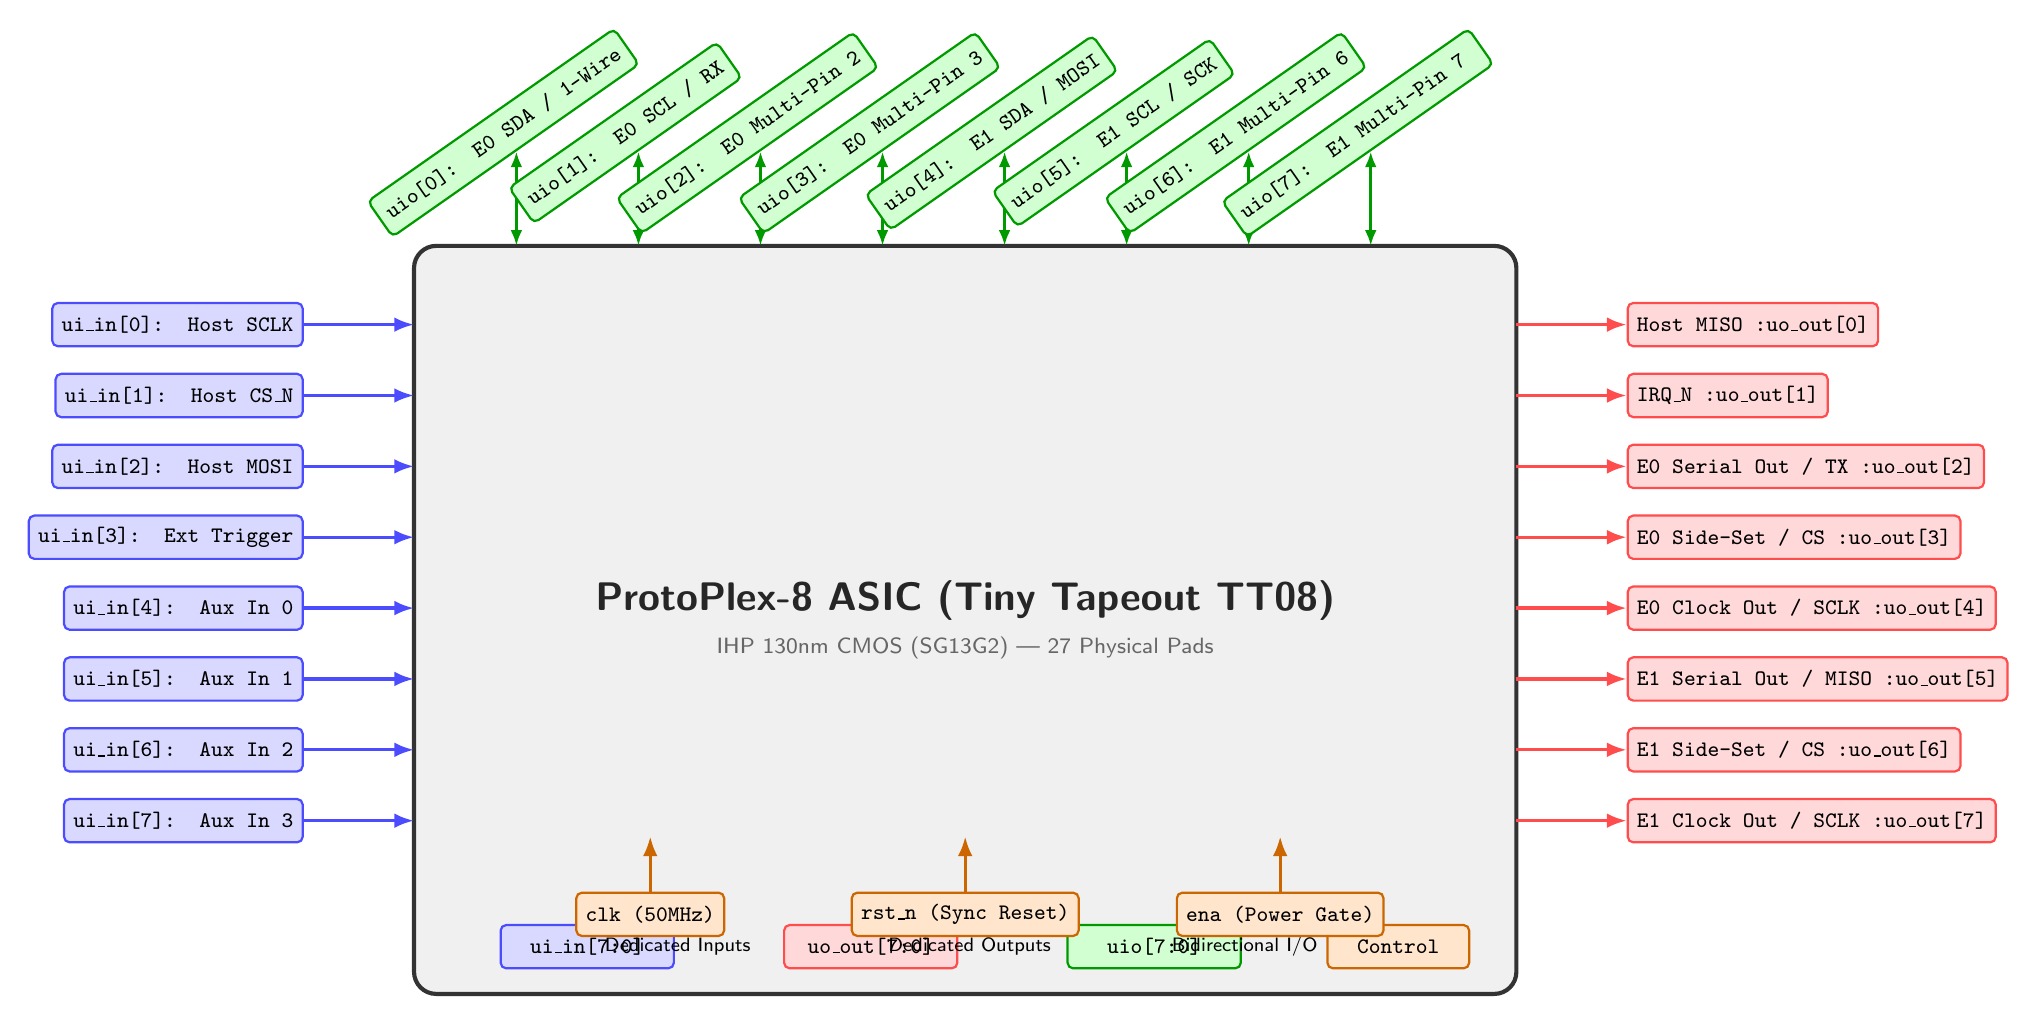
\begin{tikzpicture}[
    pin_in/.style={fill=blue!15, draw=blue!70, thick, rounded corners=2pt, minimum height=0.55cm, font=\footnotesize\ttfamily},
    pin_out/.style={fill=red!15, draw=red!70, thick, rounded corners=2pt, minimum height=0.55cm, font=\footnotesize\ttfamily},
    pin_io/.style={fill=green!18, draw=green!60!black, thick, rounded corners=2pt, minimum height=0.55cm, font=\footnotesize\ttfamily},
    pin_pwr/.style={fill=orange!20, draw=orange!80!black, thick, rounded corners=2pt, minimum height=0.55cm, font=\footnotesize\ttfamily},
    label_txt/.style={font=\scriptsize\sffamily, align=left}
]

% Chip body
\draw[fill=gray!12, draw=black!80, line width=1.5pt, rounded corners=8pt] (0,0) rectangle (14, 9.5);
\node[font=\Large\bfseries\sffamily, text=black!85] at (7, 5.0) {ProtoPlex-8 ASIC (Tiny Tapeout TT08)};
\node[font=\footnotesize\sffamily, text=gray!80!black] at (7, 4.4) {IHP 130nm CMOS (SG13G2) --- 27 Physical Pads};

% Legend
\node[pin_in, minimum width=2.2cm] at (2.2, 0.6) {ui\_in[7:0]};
\node[font=\scriptsize\sffamily, right=0.1cm of {2.2, 0.6}] {Dedicated Inputs};
\node[pin_out, minimum width=2.2cm] at (5.8, 0.6) {uo\_out[7:0]};
\node[font=\scriptsize\sffamily, right=0.1cm of {5.8, 0.6}] {Dedicated Outputs};
\node[pin_io, minimum width=2.2cm] at (9.4, 0.6) {uio[7:0]};
\node[font=\scriptsize\sffamily, right=0.1cm of {9.4, 0.6}] {Bidirectional I/O};
\node[pin_pwr, minimum width=1.8cm] at (12.5, 0.6) {Control};

% Left side: ui_in[7:0] (Inputs)
\foreach \i/\desc in {
    0/{ui\_in[0]: Host SCLK},
    1/{ui\_in[1]: Host CS\_N},
    2/{ui\_in[2]: Host MOSI},
    3/{ui\_in[3]: Ext Trigger},
    4/{ui\_in[4]: Aux In 0},
    5/{ui\_in[5]: Aux In 1},
    6/{ui\_in[6]: Aux In 2},
    7/{ui\_in[7]: Aux In 3}
} {
    \draw[-{Latex[length=2.5mm]}, blue!70, line width=1.2pt] (-1.4, 8.5 - \i*0.9) -- (0, 8.5 - \i*0.9);
    \node[pin_in, anchor=east] at (-1.4, 8.5 - \i*0.9) {\desc};
}

% Right side: uo_out[7:0] (Outputs)
\foreach \i/\desc in {
    0/{Host MISO :uo\_out[0]},
    1/{IRQ\_N :uo\_out[1]},
    2/{E0 Serial Out / TX :uo\_out[2]},
    3/{E0 Side-Set / CS :uo\_out[3]},
    4/{E0 Clock Out / SCLK :uo\_out[4]},
    5/{E1 Serial Out / MISO :uo\_out[5]},
    6/{E1 Side-Set / CS :uo\_out[6]},
    7/{E1 Clock Out / SCLK :uo\_out[7]}
} {
    \draw[{Latex[length=2.5mm]}-, red!70, line width=1.2pt] (15.4, 8.5 - \i*0.9) -- (14, 8.5 - \i*0.9);
    \node[pin_out, anchor=west] at (15.4, 8.5 - \i*0.9) {\desc};
}

% Top side: uio[7:0] (Bidirectional)
\foreach \i/\desc in {
    0/{uio[0]: E0 SDA / 1-Wire},
    1/{uio[1]: E0 SCL / RX},
    2/{uio[2]: E0 Multi-Pin 2},
    3/{uio[3]: E0 Multi-Pin 3},
    4/{uio[4]: E1 SDA / MOSI},
    5/{uio[5]: E1 SCL / SCK},
    6/{uio[6]: E1 Multi-Pin 6},
    7/{uio[7]: E1 Multi-Pin 7}
} {
    \draw[{Latex[length=2mm]}-{Latex[length=2mm]}, green!60!black, line width=1.2pt] (1.3 + \i*1.55, 10.7) -- (1.3 + \i*1.55, 9.5);
    \node[pin_io, anchor=south, rotate=35, align=left] at (1.3 + \i*1.55, 10.7) {\desc};
}

% Bottom side: Power / Control
\draw[-{Latex[length=2.5mm]}, orange!80!black, line width=1.2pt] (3.0, 1.3) -- (3.0, 2.0);
\node[pin_pwr, anchor=north] at (3.0, 1.3) {clk (50MHz)};

\draw[-{Latex[length=2.5mm]}, orange!80!black, line width=1.2pt] (7.0, 1.3) -- (7.0, 2.0);
\node[pin_pwr, anchor=north] at (7.0, 1.3) {rst\_n (Sync Reset)};

\draw[-{Latex[length=2.5mm]}, orange!80!black, line width=1.2pt] (11.0, 1.3) -- (11.0, 2.0);
\node[pin_pwr, anchor=north] at (11.0, 1.3) {ena (Power Gate)};

\end{tikzpicture}
\end{document}
